\documentclass[border=1cm,tikz]{standalone}
\usepackage{graphicx}

\begin{document}

\begin{tikzpicture}

\node (back) at (0,0) {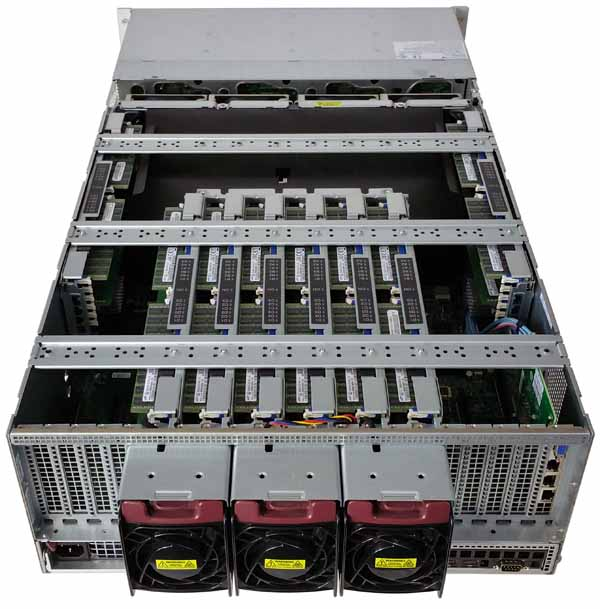
\includegraphics[width=0.75\textwidth]{fats/image-fat_back}};
\node (back) at (0,0) {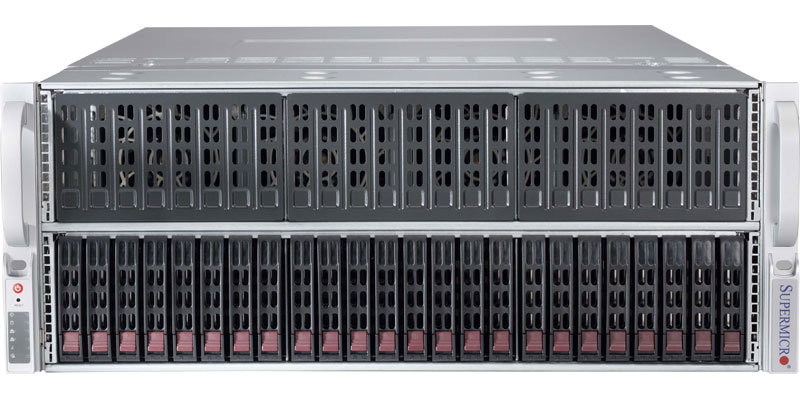
\includegraphics[width=0.75\textwidth]{fats/image-fat_front}};
% \node (back) at (0,0) {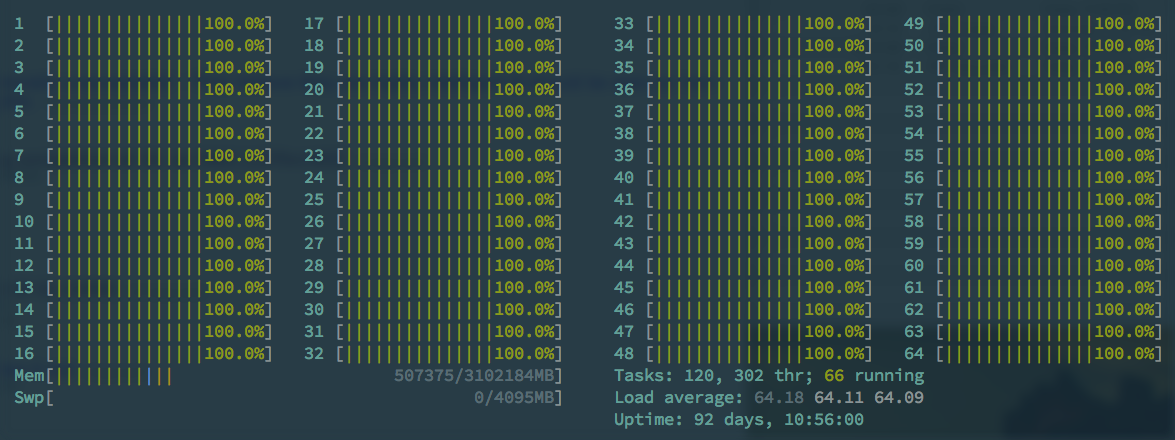
\includegraphics[width=0.75\textwidth]{fats/image-fat_htop}};
\node (back) at (0,0) {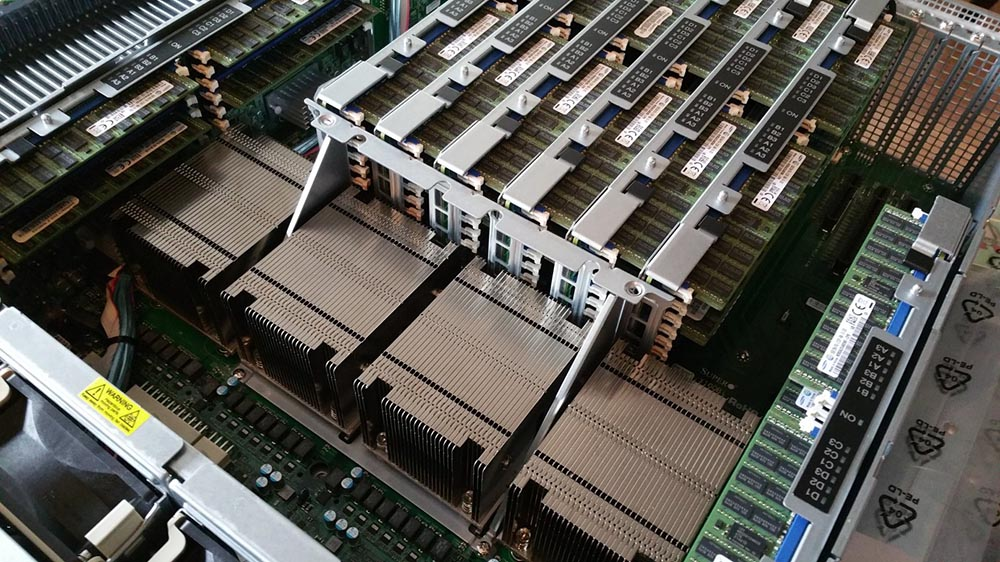
\includegraphics[width=0.75\textwidth]{fats/image-fat_inside}};
\node (back) at (0,0) {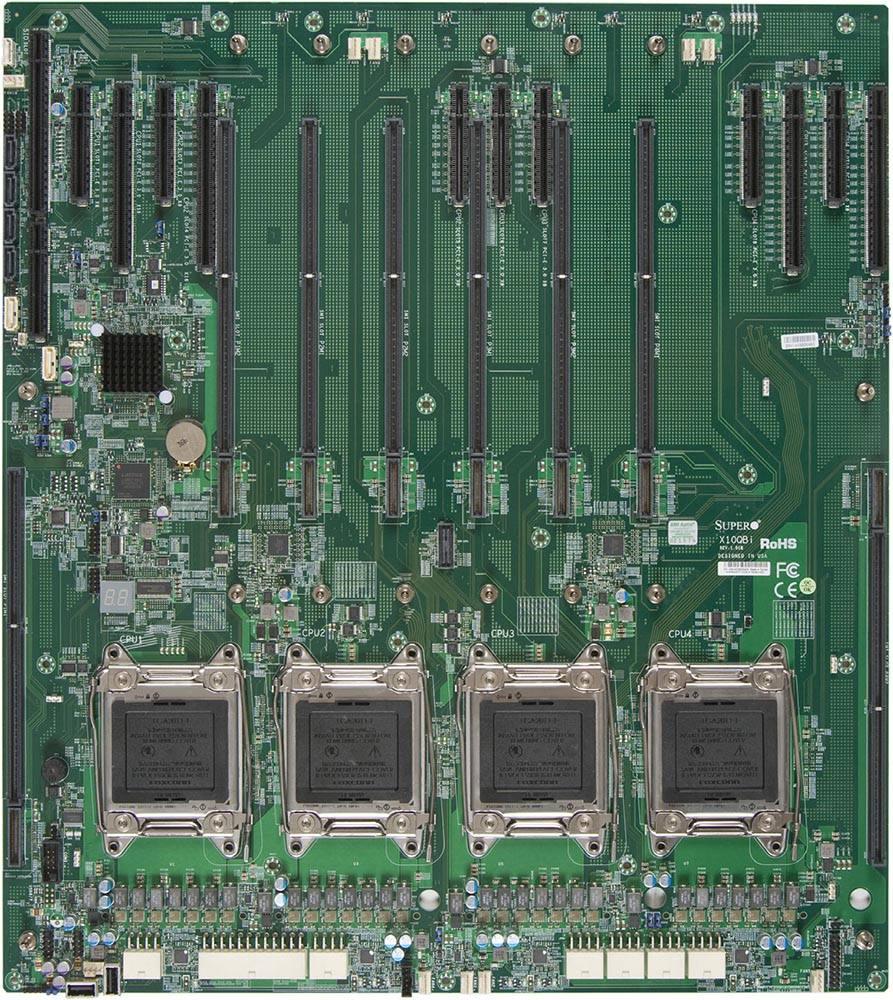
\includegraphics[width=0.75\textwidth]{fats/image-fat_mobo}};
\node (back) at (0,0) {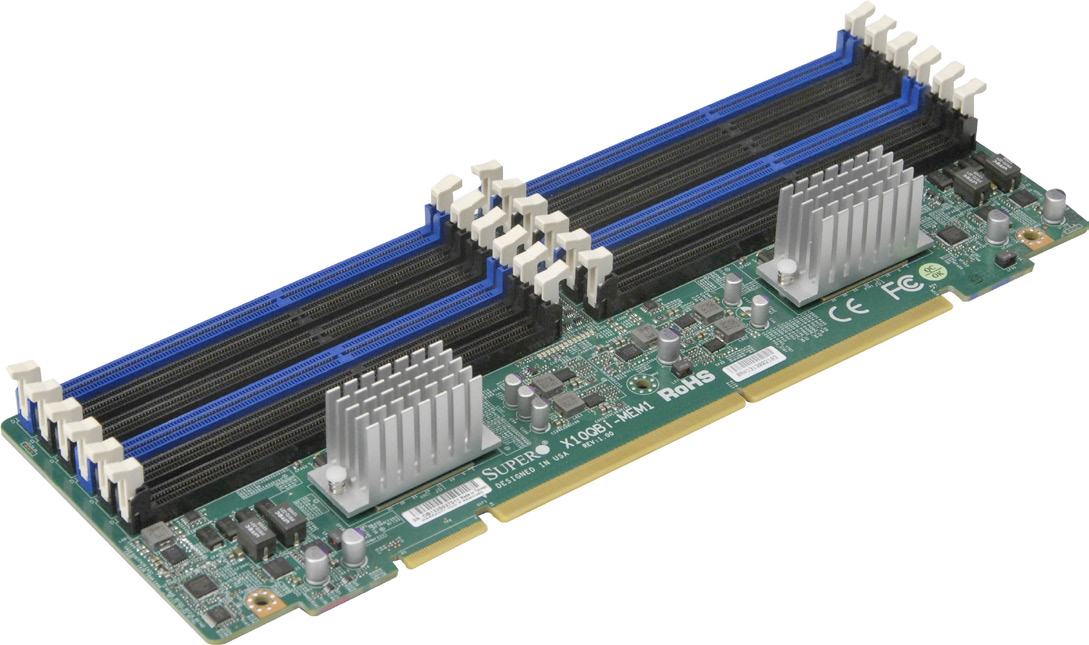
\includegraphics[width=0.75\textwidth]{fats/image-fat_riser}};



% \begin{scope}[x={(image.south east)}, y={(image.north west)}]
%     \node at (0.5,1.04) {\large 2$\times$1 reconstruction $\Rightarrow\chi^{xxx}_{\mathrm{2\times 1}}\ne 0$};
%     \node[rotate=15.5] at (0.82,0.57) {\large ${\mathcal{C}}(z) = 1$};
%     \draw[color=red, thick, dashed] (0,0.40) -- (1,0.57);
%     \node[rotate=15.5] at (0.85,0.51) {\large ${\mathcal{C}}(z) = 0$};
%     \node at (0.5,-0.03) {\large H-terminated $\Rightarrow\chi^{xxx}_{\mathrm{H}}= 0$};
% \end{scope}

\end{tikzpicture}

\end{document}
